%%PREAMBLE %%%%%%%%%%%%%%%%%%%%%%%%%%%%
\documentclass[10pt, a4paper]{article}% size of txt = 10pt
\usepackage[top= 2cm,
			bottom = 2cm,
			left = 1.7cm,
			right = 1.7cm,
			footskip = 0.5cm,
			headsep = 0cm,
			headheight = 0cm
					]{geometry}
\usepackage{amsmath} % math packages
\usepackage{amsfonts}% math packages
\usepackage{amssymb} % math packages
\usepackage{graphicx} %package for including graphics
\usepackage{array}
\usepackage[thinlines]{easytable}
\usepackage{float}
\usepackage[section]{placeins}
\usepackage[hidelinks]{hyperref}
\usepackage[shortlabels]{enumitem}
\usepackage{svg}
\usepackage{bigstrut}
\usepackage{wrapfig,lipsum,booktabs}
\usepackage{subcaption}
\usepackage{xfrac}
\usepackage{pdfpages}
\usepackage{listings}
\usepackage{xcolor}

\usepackage{listings}
\usepackage{color} %red, green, blue, yellow, cyan, magenta, black, white
\usepackage{pdfpages}
\definecolor{mygreen}{RGB}{28,172,0} % color values Red, Green, Blue
\definecolor{mylilas}{RGB}{170,55,241}

\definecolor{codegreen}{rgb}{0,0.6,0}
\definecolor{codegray}{rgb}{0.5,0.5,0.5}
\definecolor{codepurple}{rgb}{0.58,0,0.82}
\definecolor{backcolour}{rgb}{1,1,1}

\lstdefinestyle{mystyle}{
    backgroundcolor=\color{backcolour},   
    commentstyle=\color{codegreen},
    keywordstyle=\color{magenta},
    numberstyle=\tiny\color{codegray},
    stringstyle=\color{codepurple},
    basicstyle=\ttfamily\footnotesize,
    breakatwhitespace=false,         
    breaklines=true,                 
    captionpos=b,                    
    keepspaces=true,                 
    numbers=left,                    
    numbersep=5pt,                  
    showspaces=false,                
    showstringspaces=false,
    showtabs=false,                  
    tabsize=2
}
\lstset{style=mystyle}


%date format
\def\mydate{\leavevmode\hbox{\twodigits\day.\twodigits\month.\the\year}}
\def\twodigits#1{\ifnum#1<10 0\fi\the#1}


\usepackage[T1]{fontenc} 
\usepackage{lmodern}
\usepackage{indentfirst}
\setlength{\parindent}{1cm}

\makeatletter
\newcommand{\thickhline}{%
    \noalign {\ifnum 0=`}\fi \hrule height 2pt
    \futurelet \reserved@a \@xhline
}
\newcolumntype{"}{@{\hskip\tabcolsep\vrule width 2pt\hskip\tabcolsep}}
\makeatother
\newcolumntype{?}{!{\vrule width 2pt}}
%%DOC ENVIROMENT%%%%%%%%%%%%%%%%%%%%%%%
\begin{document}
\tableofcontents

\section{Základy tvorby programů}

\includepdf[pages =-]{mspr01.pdf}
\section{Základy tvorby programů-otázky}
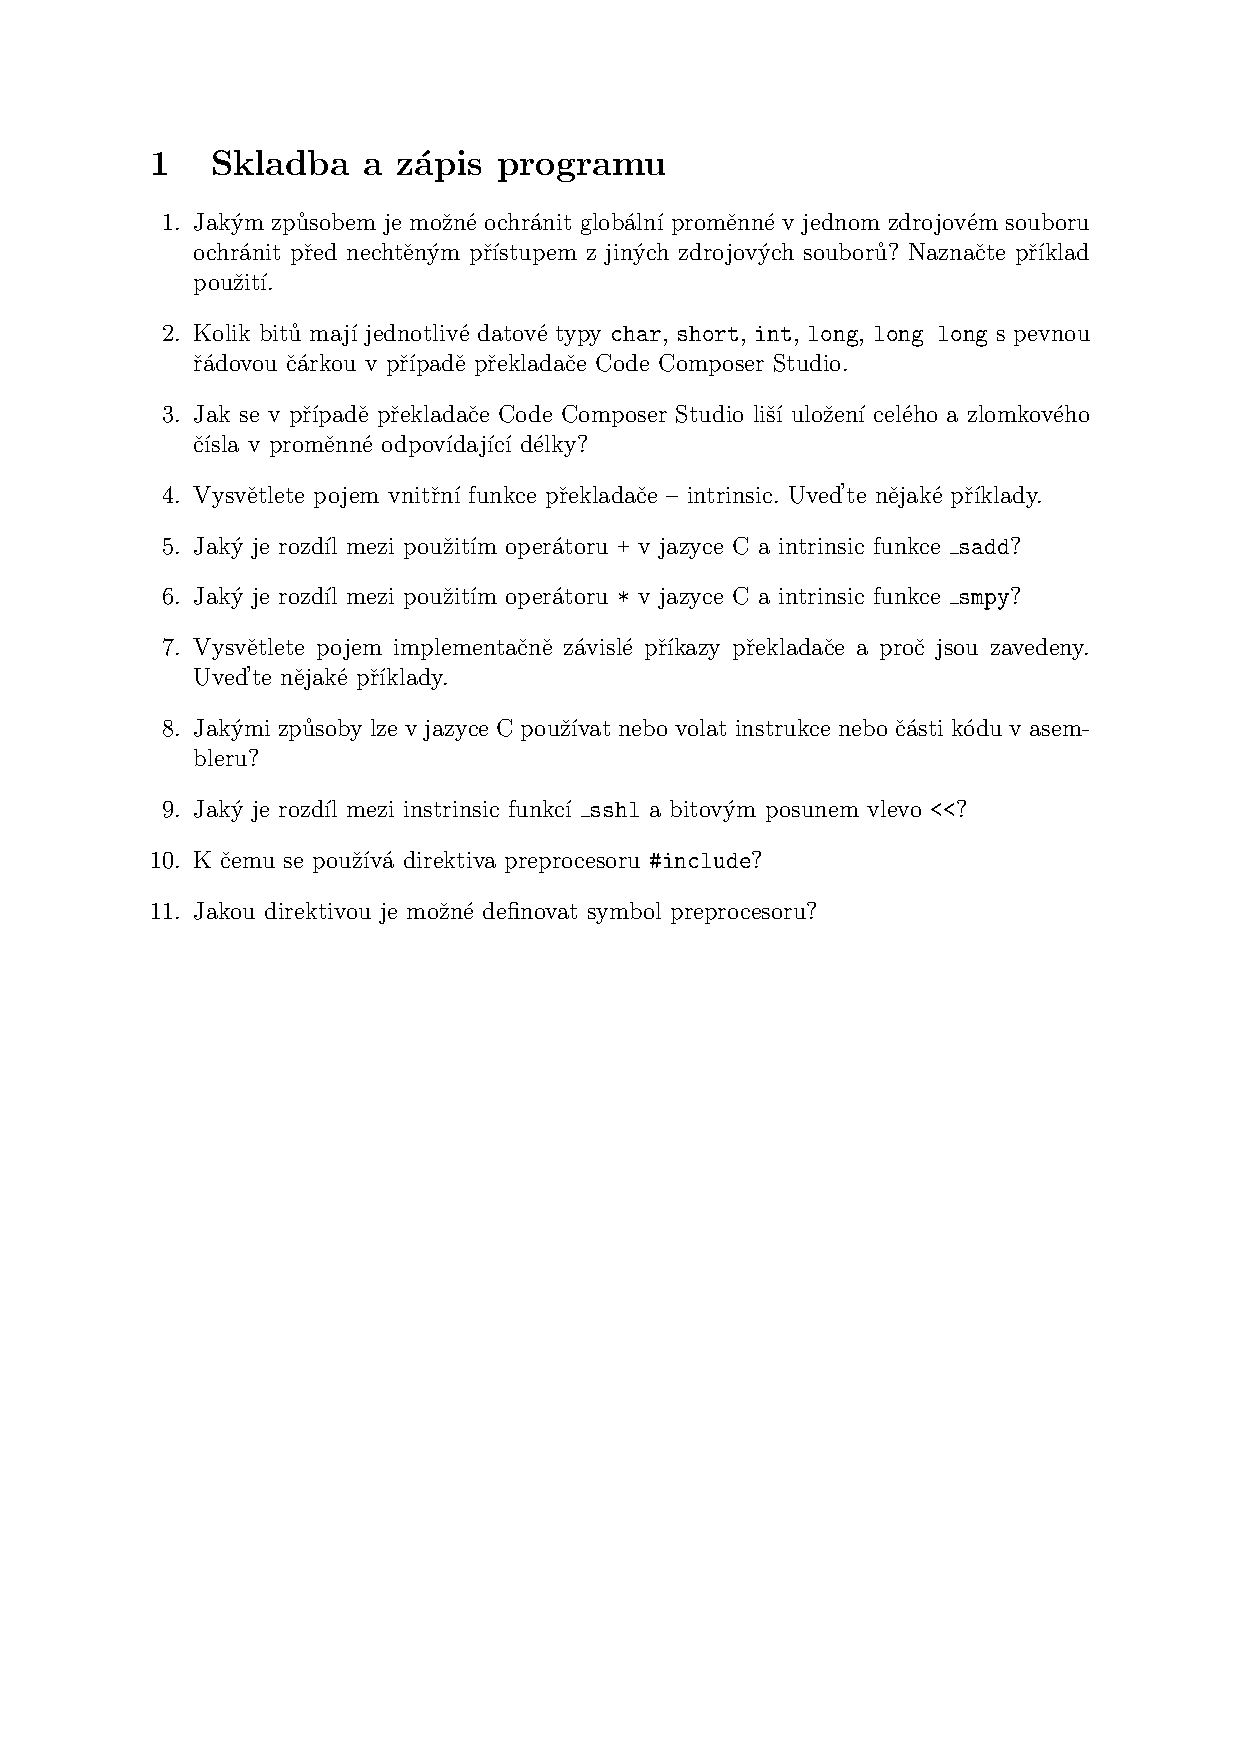
\includepdf[pages =-]{mspr-q01.pdf}
\section{Operační systémy reálného času}
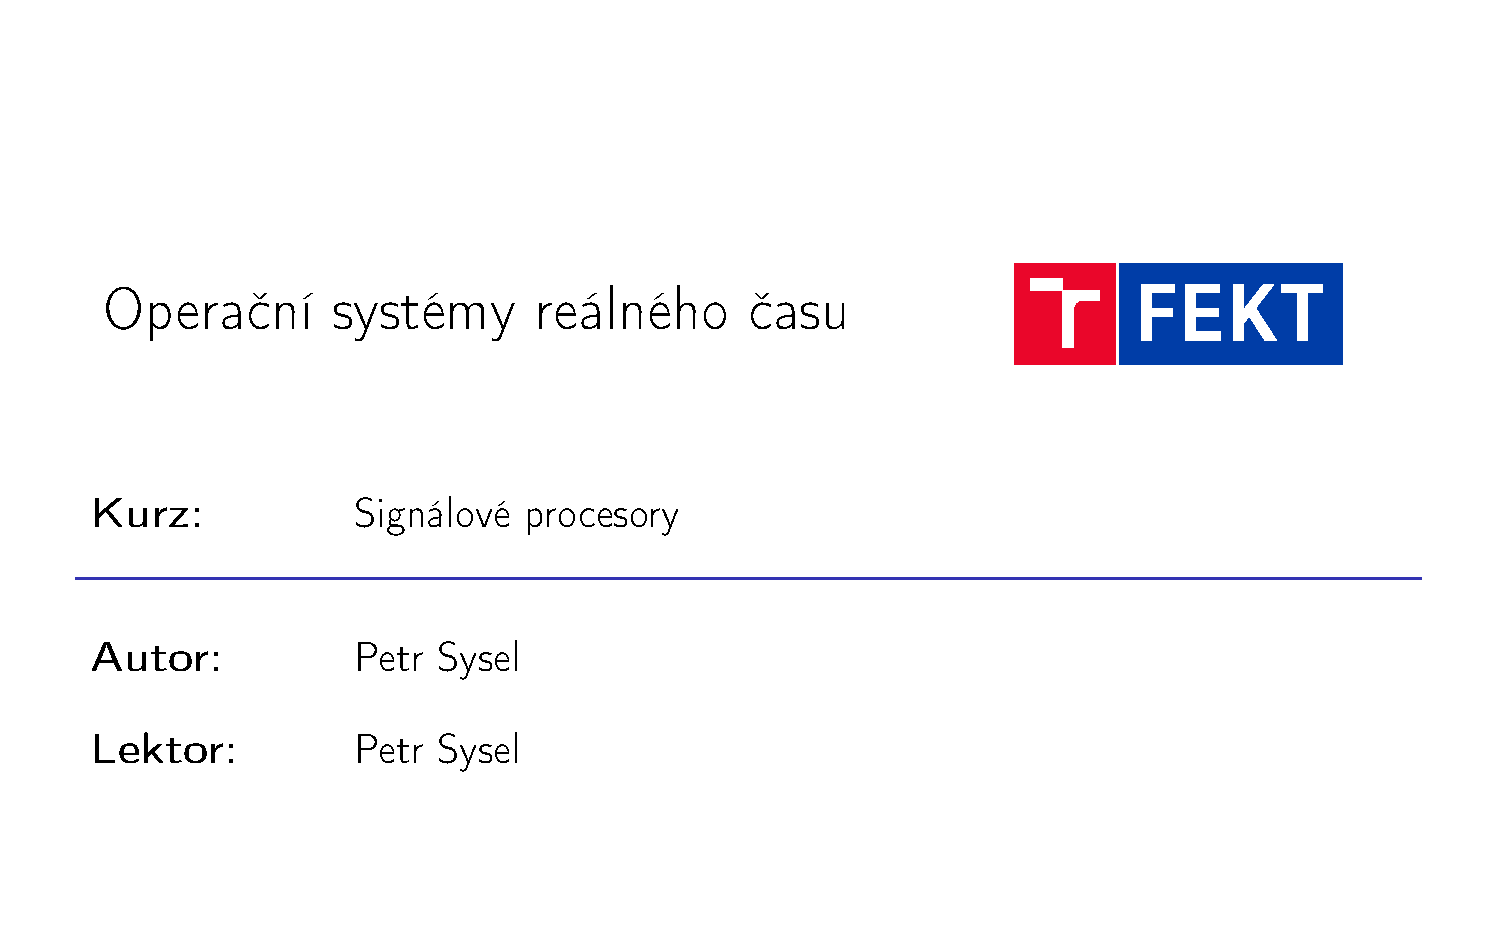
\includepdf[pages =-]{04-dspbios.pdf}
\section{Operační systémy reálného času-otázky}
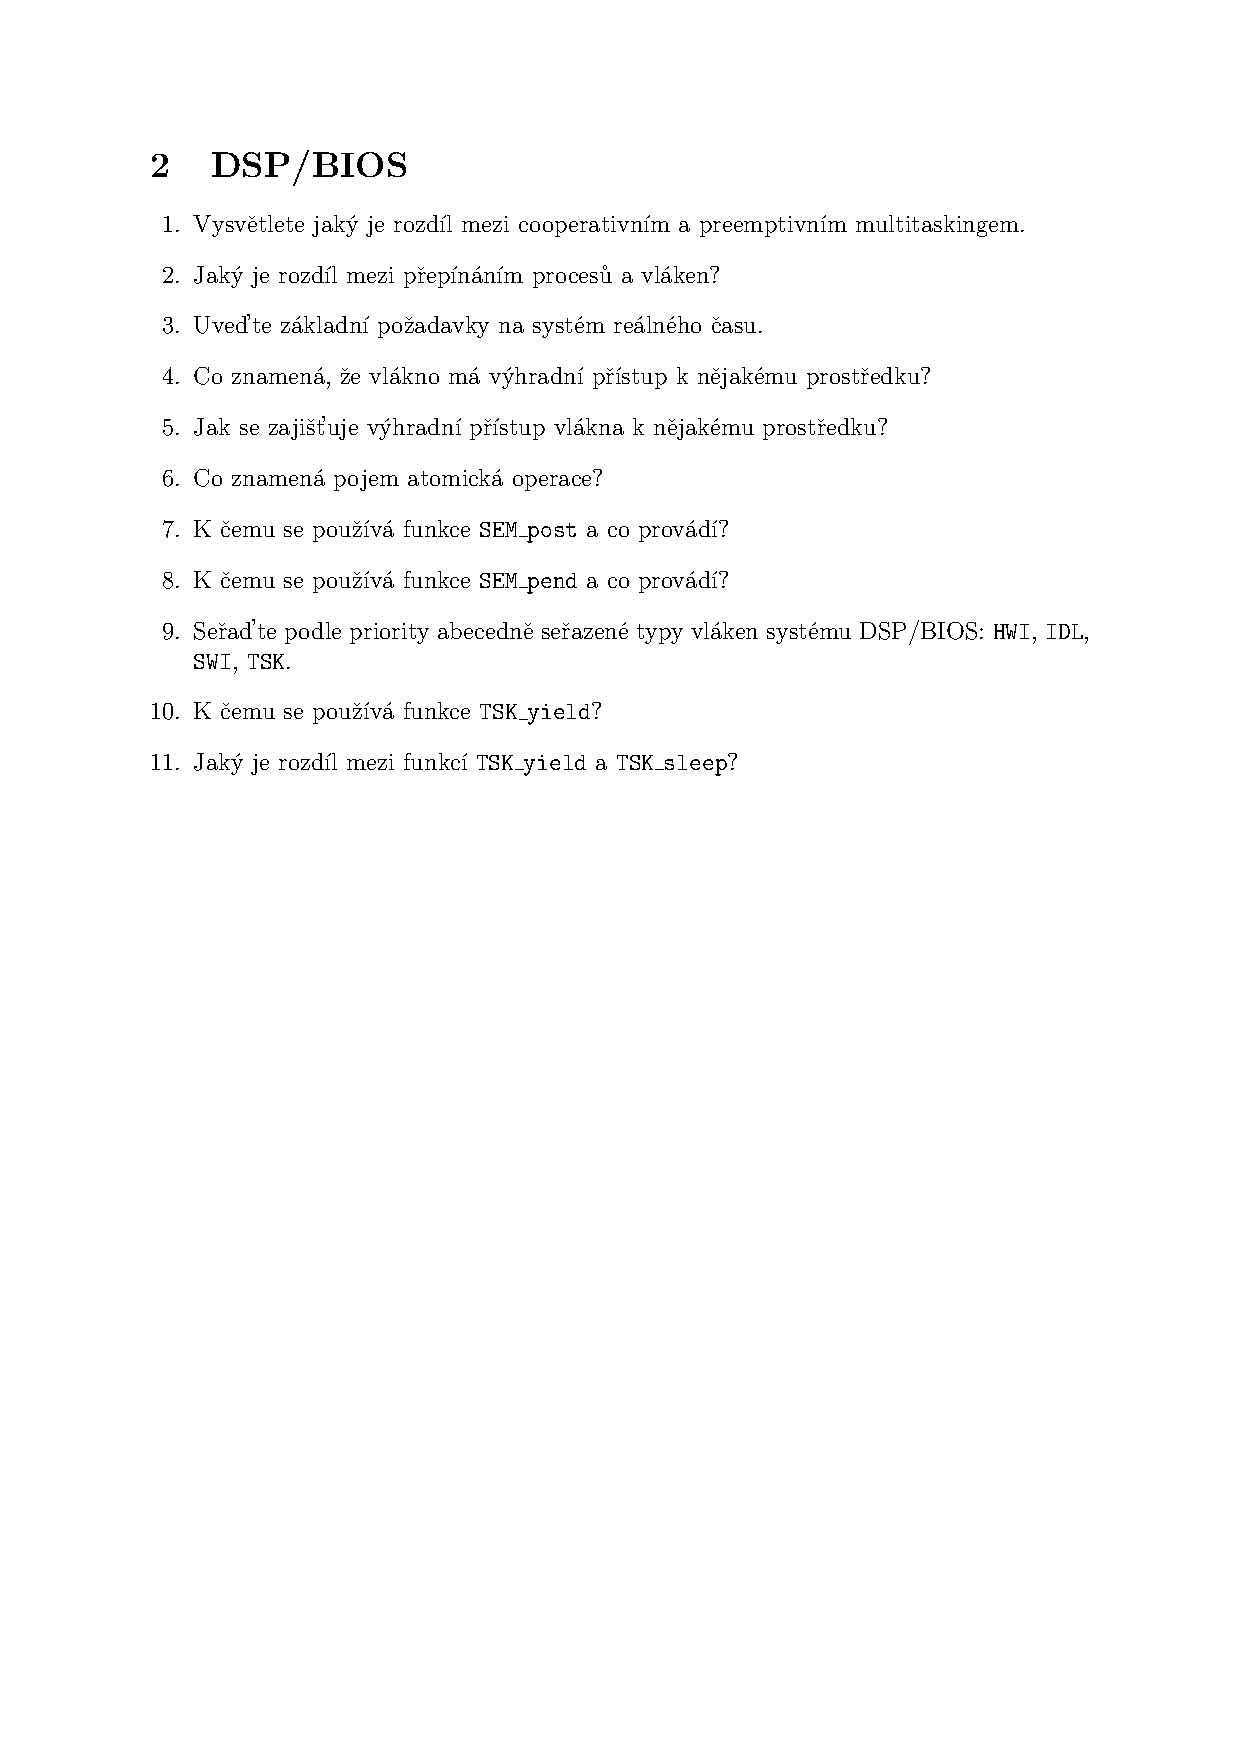
\includepdf[pages =-]{mspr-q02.pdf}
\section{Možnosti adresování a realizace kruhové paměti}
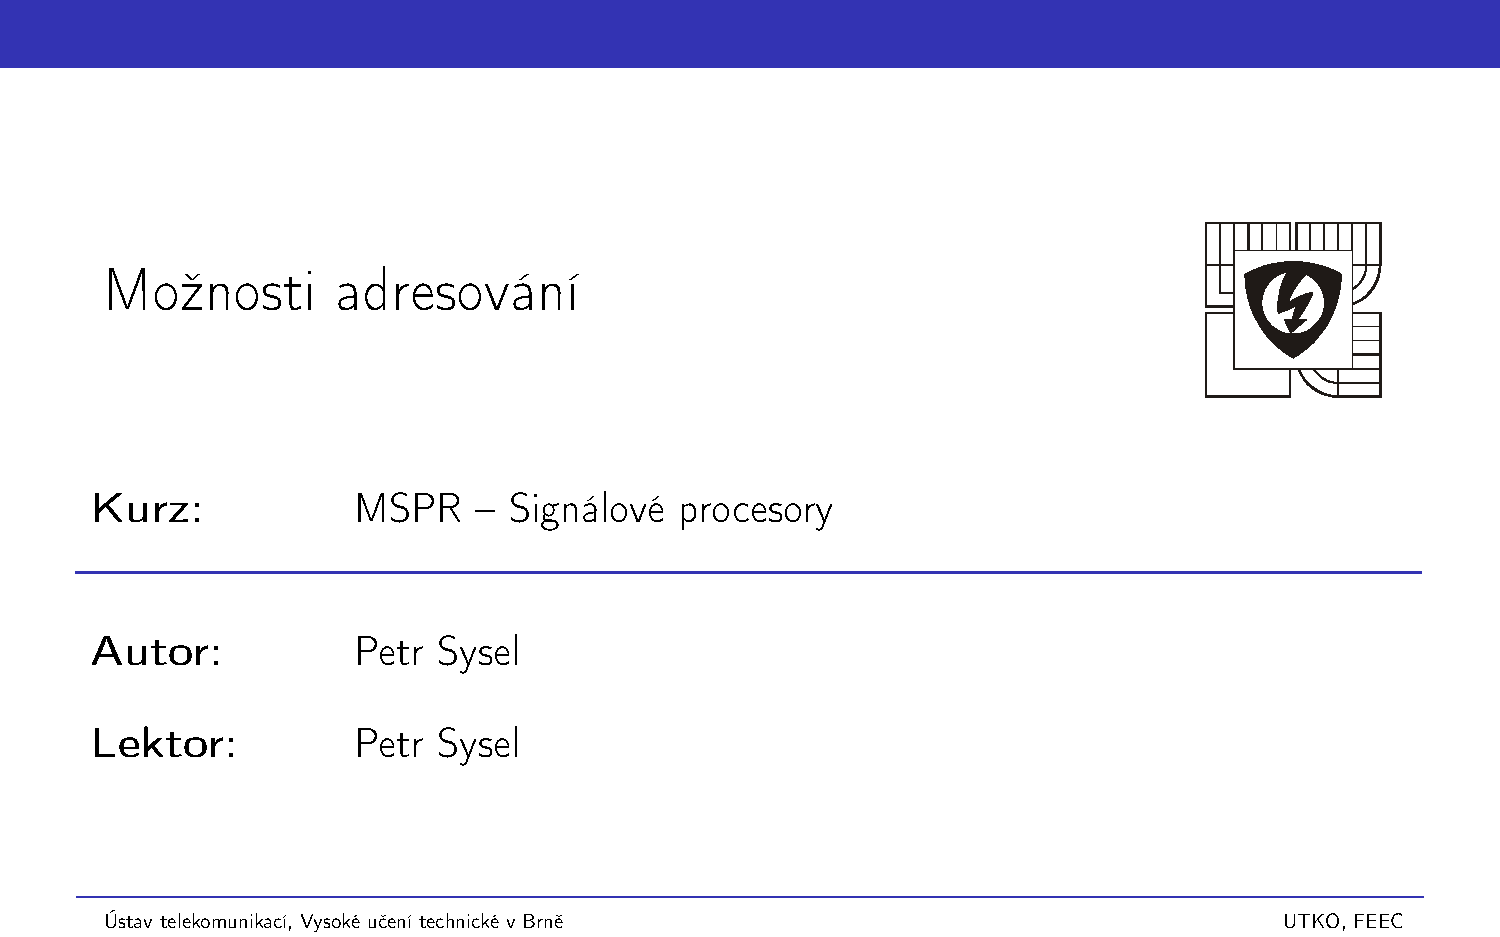
\includepdf[pages =-]{mspr-adresovani.pdf}
\section{Možnosti adresování a realizace kruhové paměti-otázky}
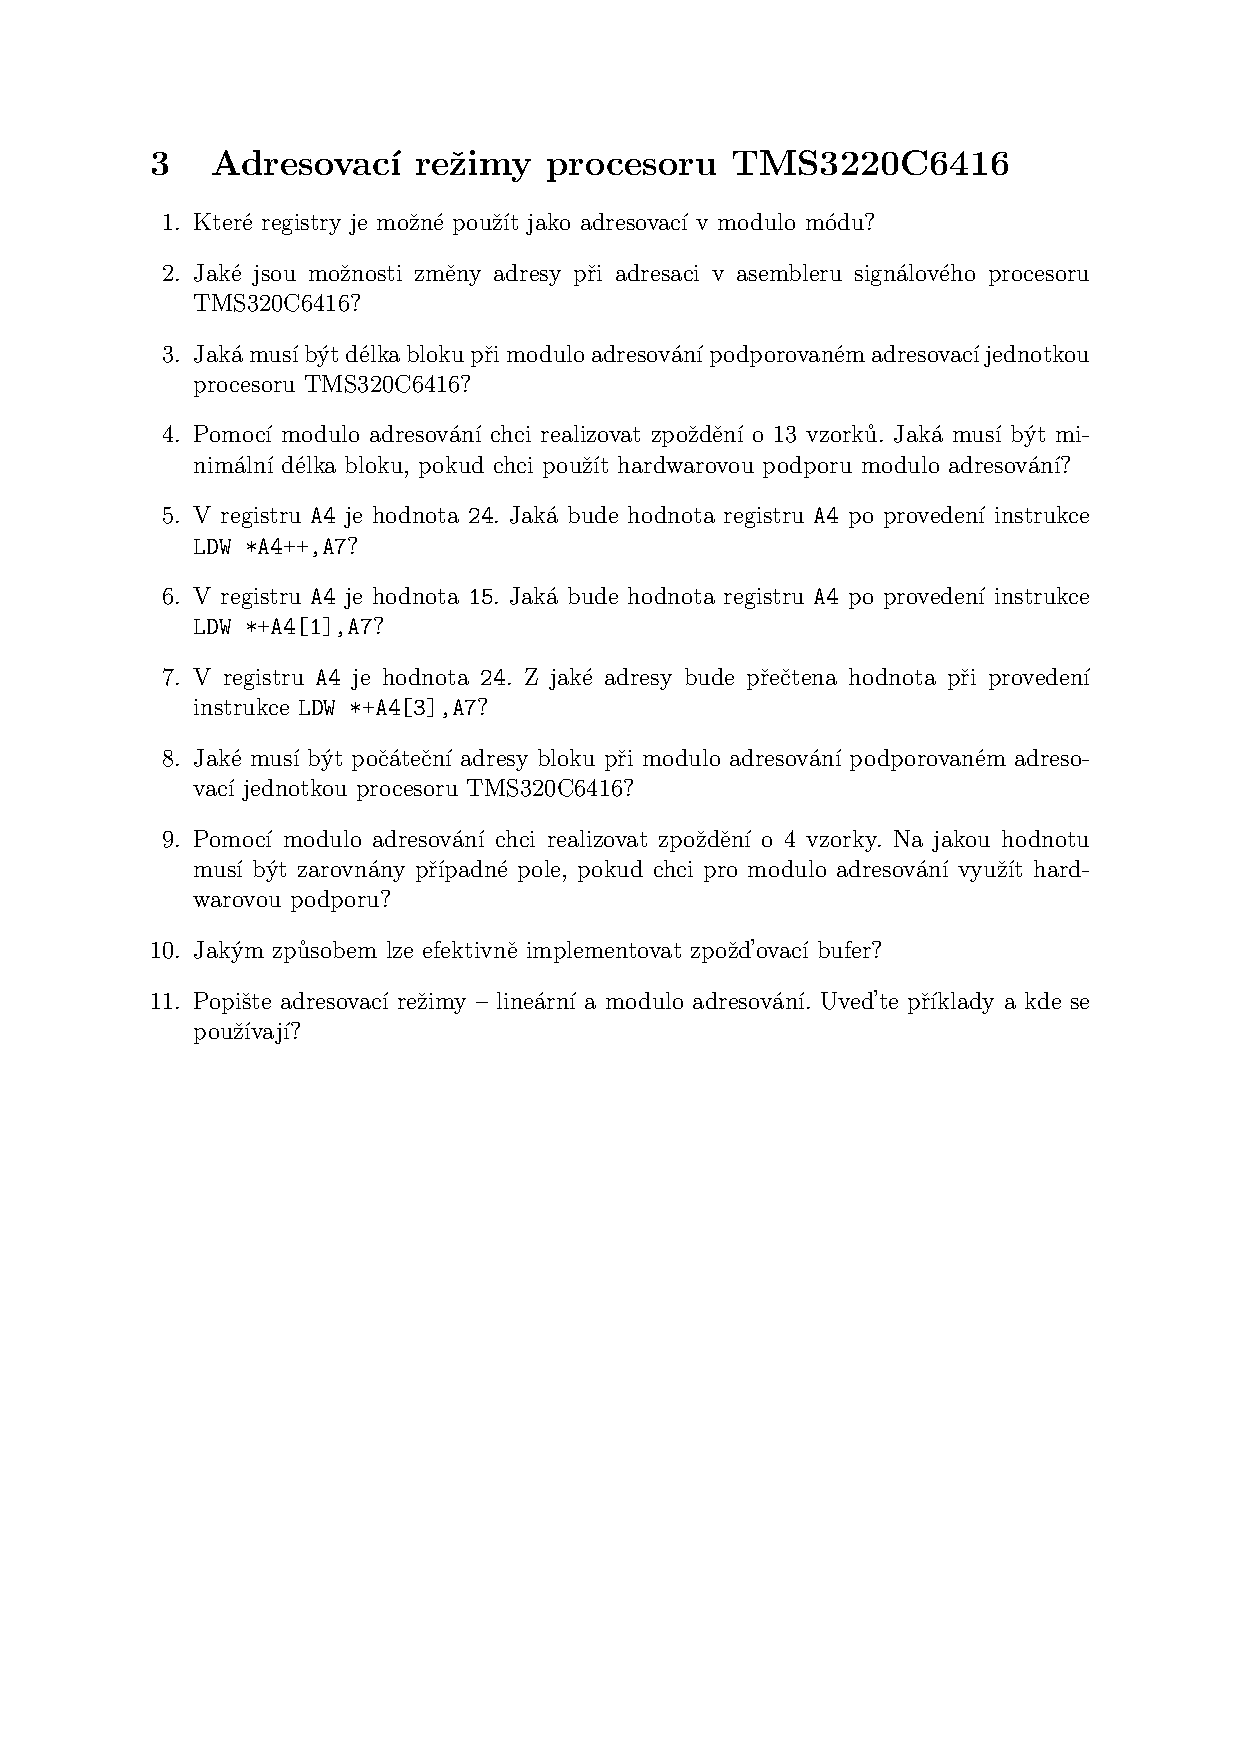
\includepdf[pages =-]{mspr-q03.pdf}
\section{Volání funkcí a přerušení programu}
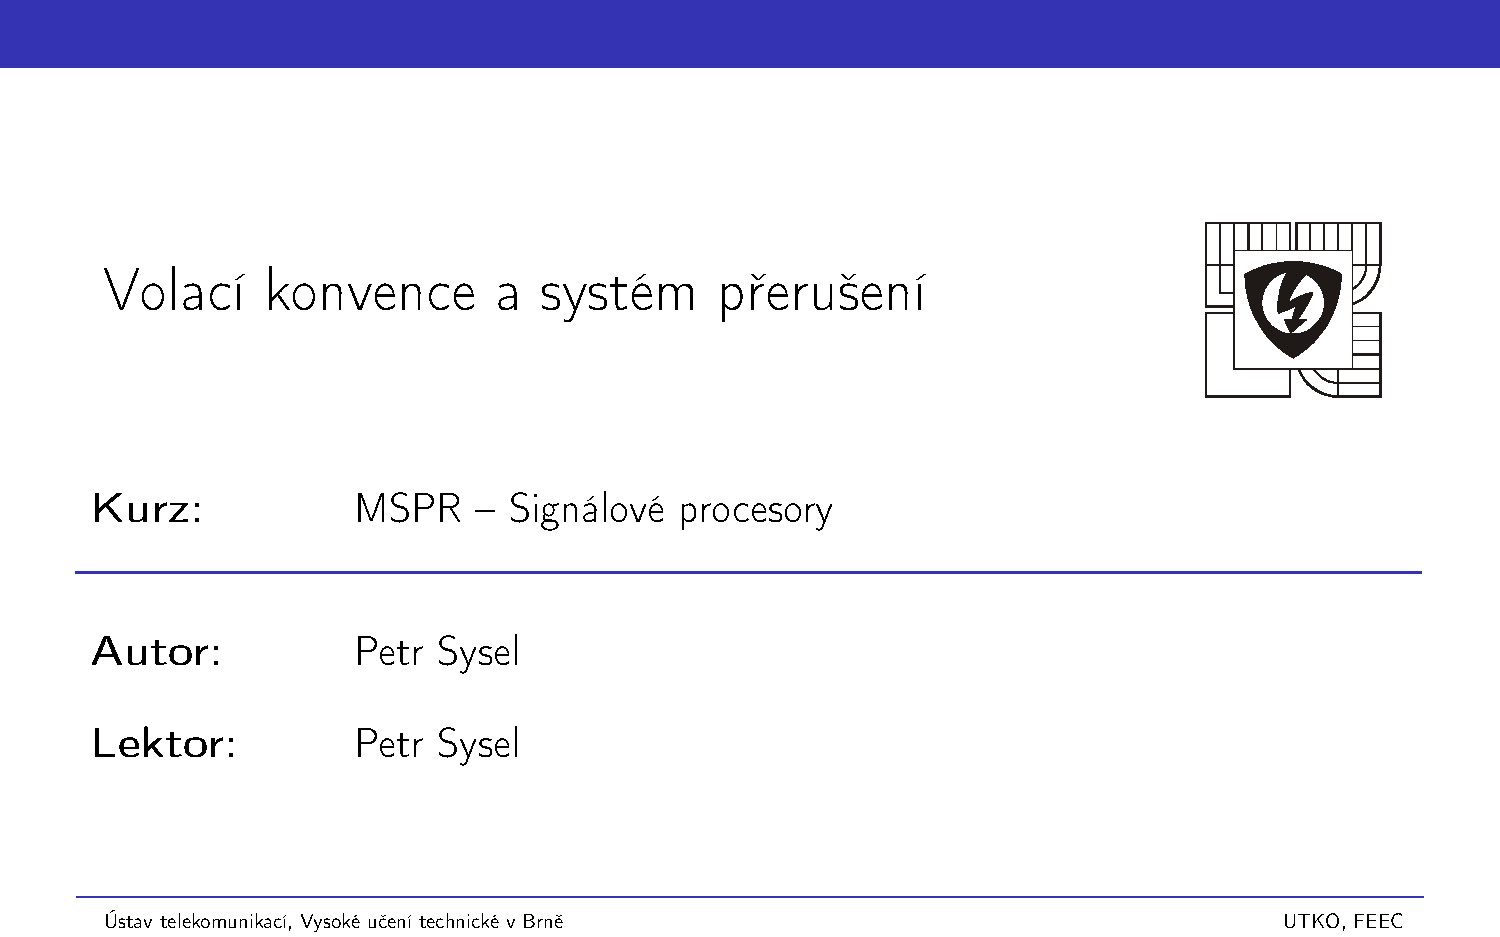
\includepdf[pages =-]{mspr-preruseni.pdf}
\section{Volání funkcí a přerušení programu-otázky}
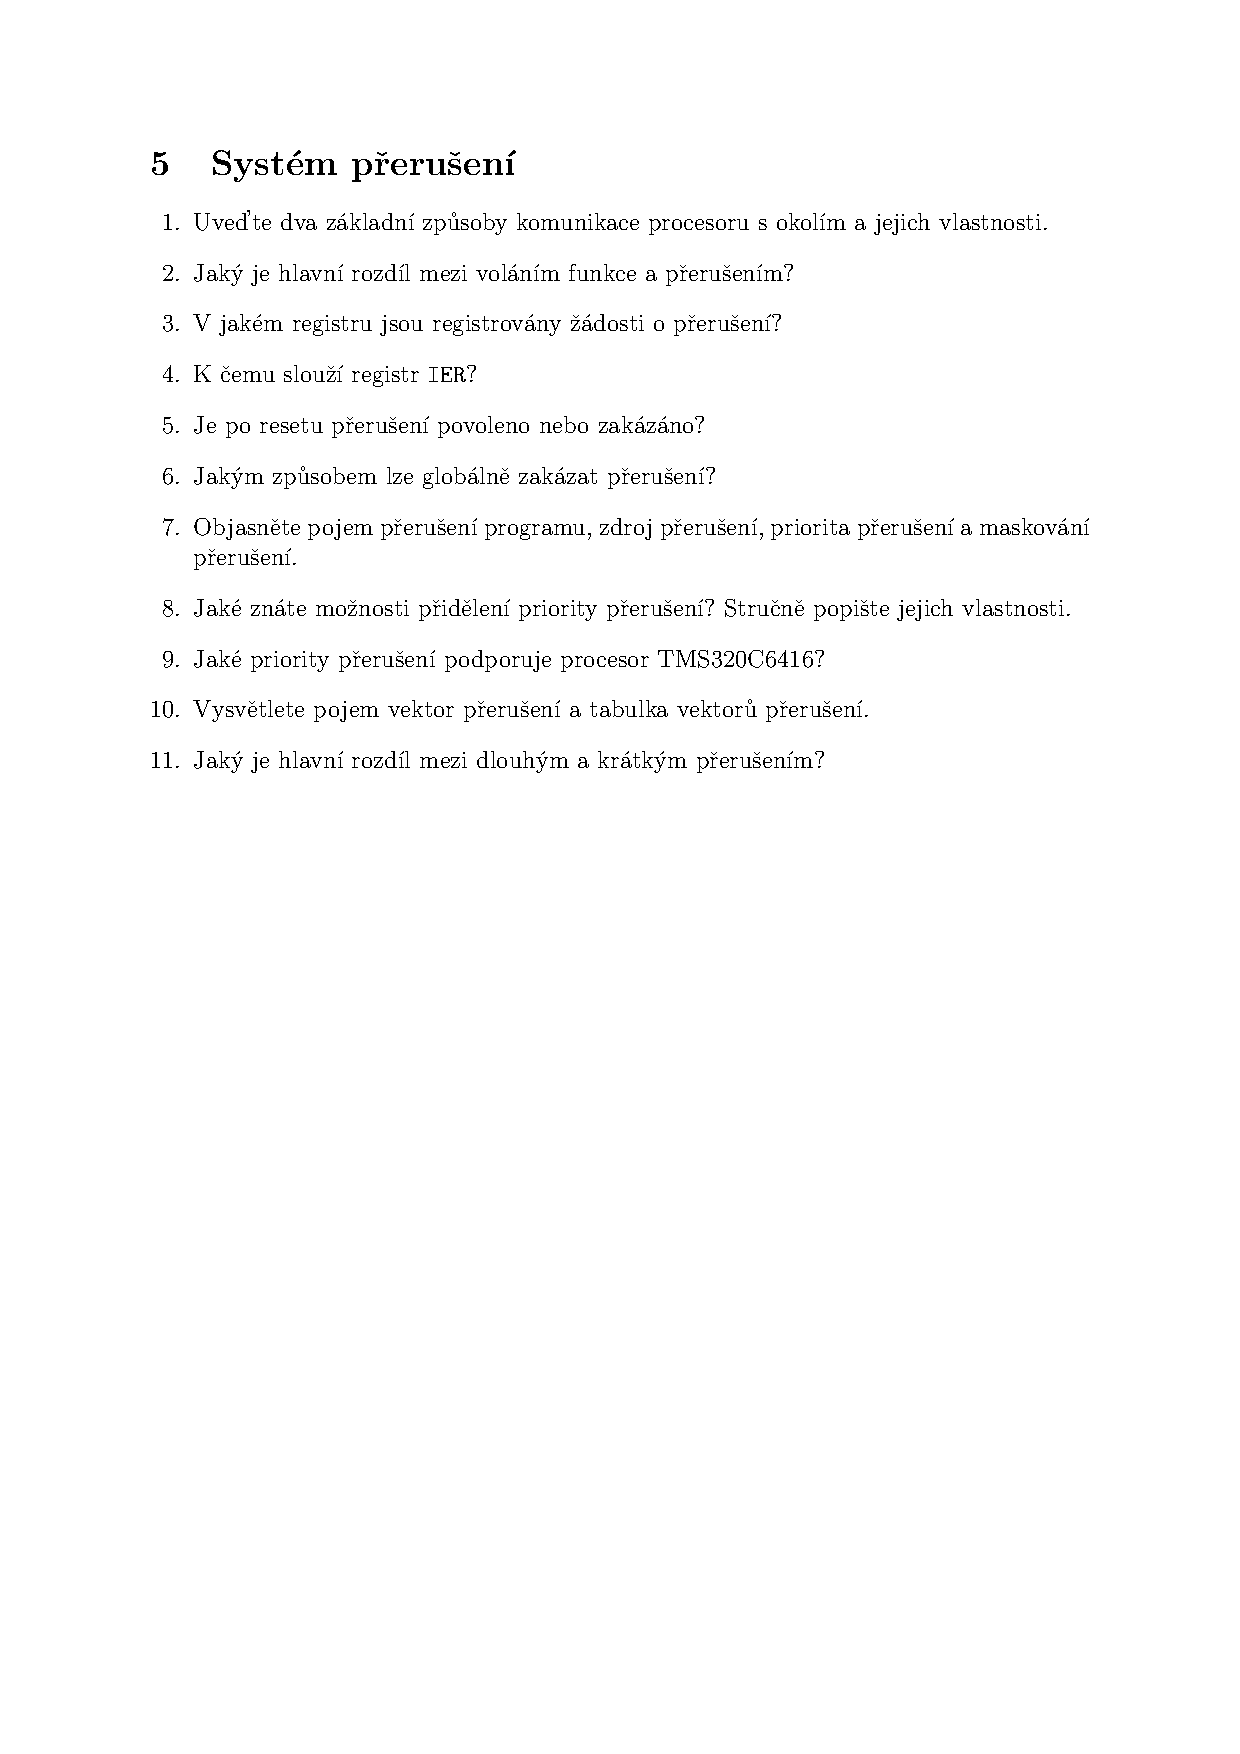
\includepdf[pages =-]{mspr-q04.pdf}
\section{Formáty čísel}

\includepdf[pages =-]{formaty.pdf}
\section{Formáty čísel-otázky}
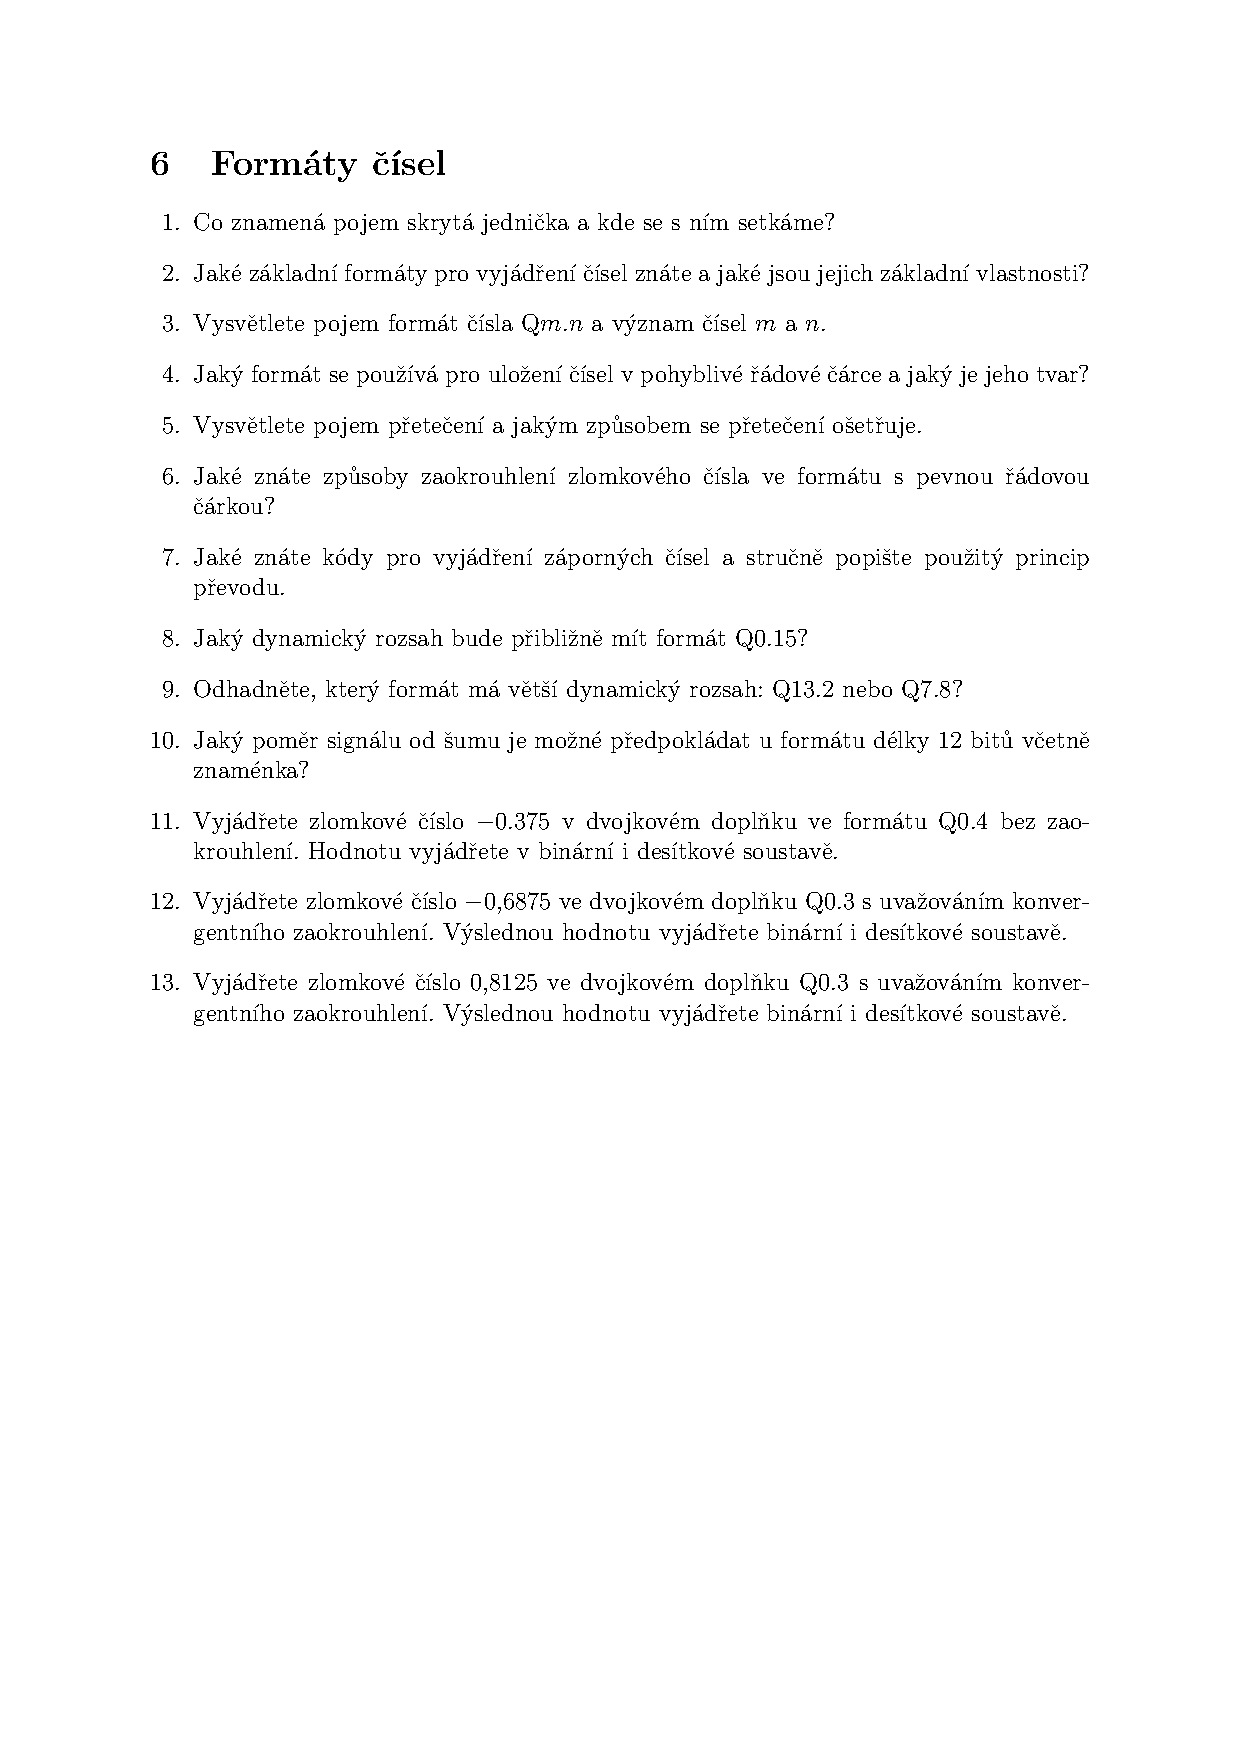
\includepdf[pages =-]{mspr-q05.pdf}
\section{Analýza číslicových systémů}

\includepdf[pages =-]{analyza.pdf}
\section{Analýza číslicových systémů-otázky}
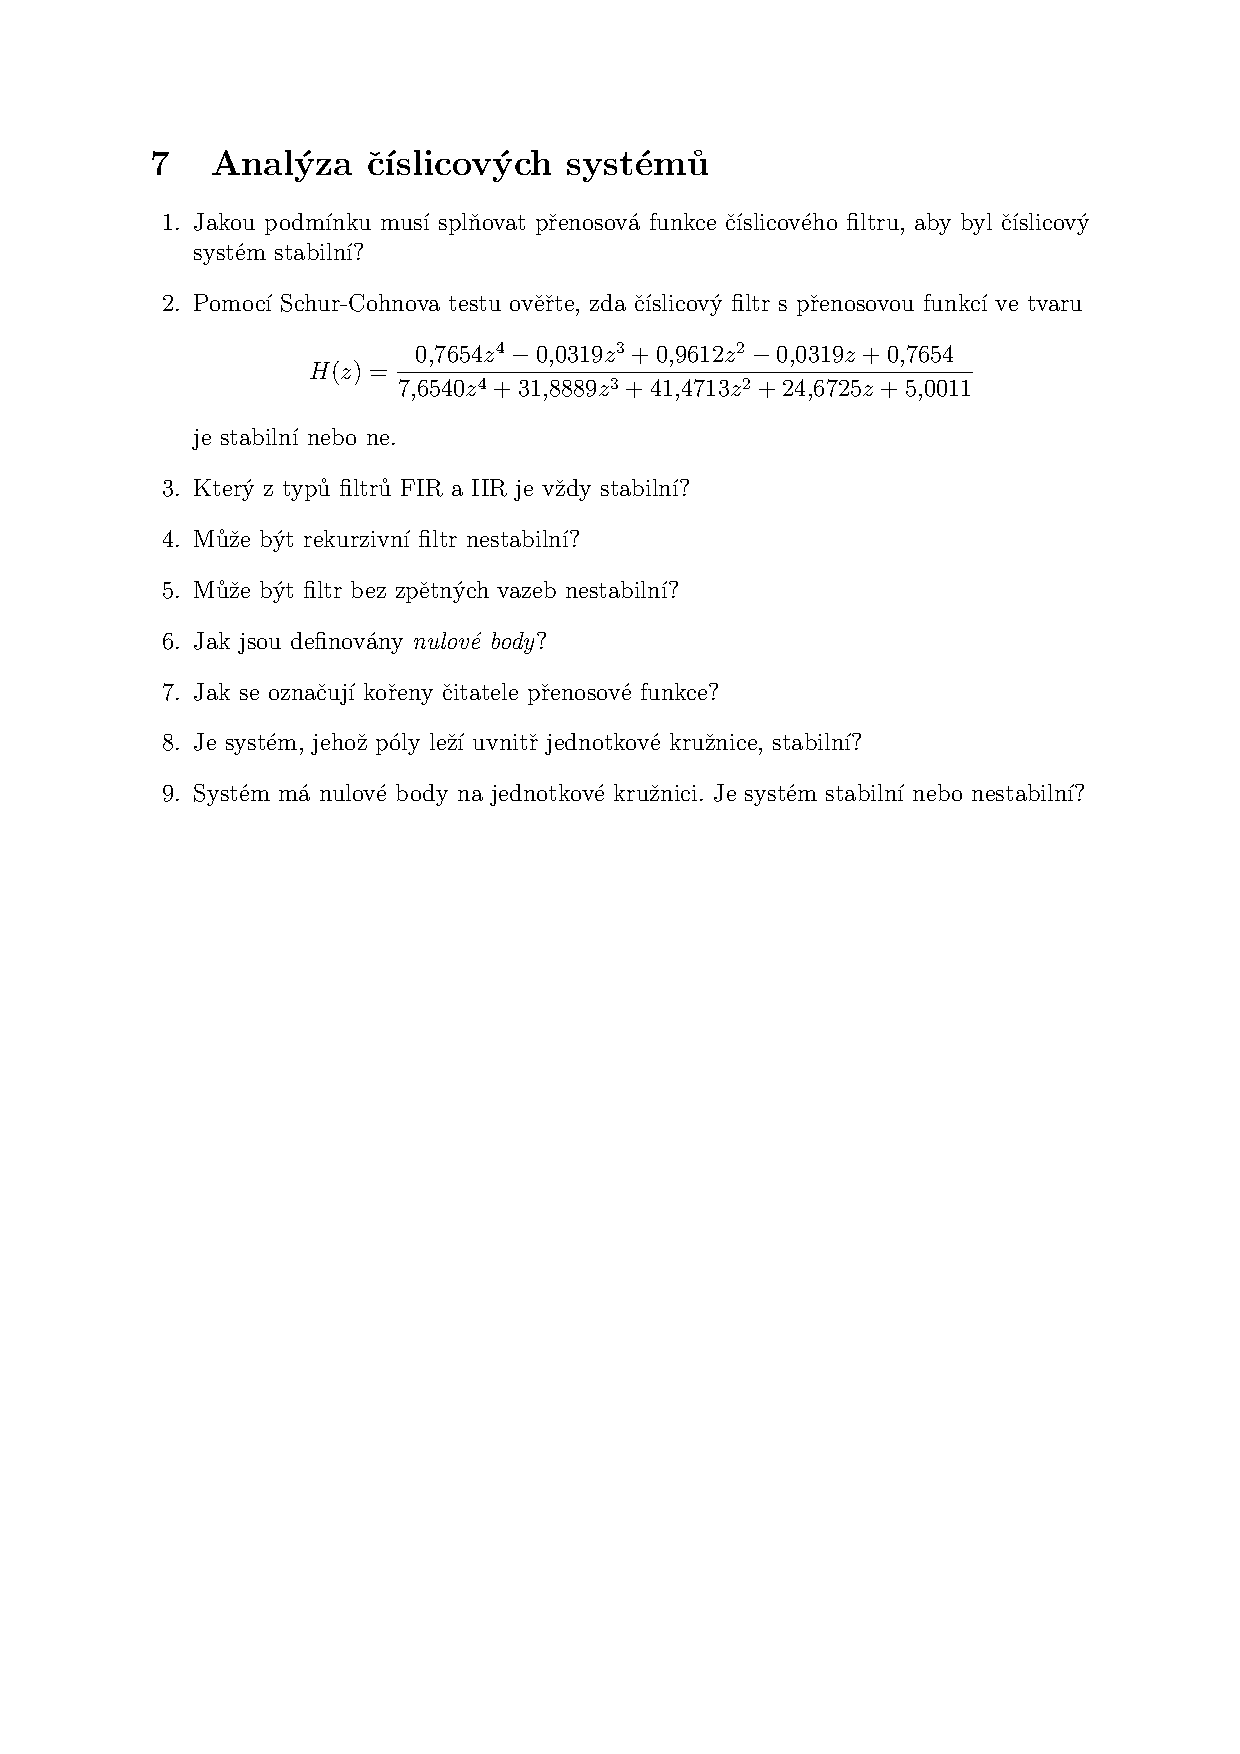
\includepdf[pages =-]{mspr-q06.pdf}
\section{Struktury implementace číslicových filtrů}

\includepdf[pages =-]{filtry.pdf}
\section{Struktury implementace číslicových filtrů-otázky}
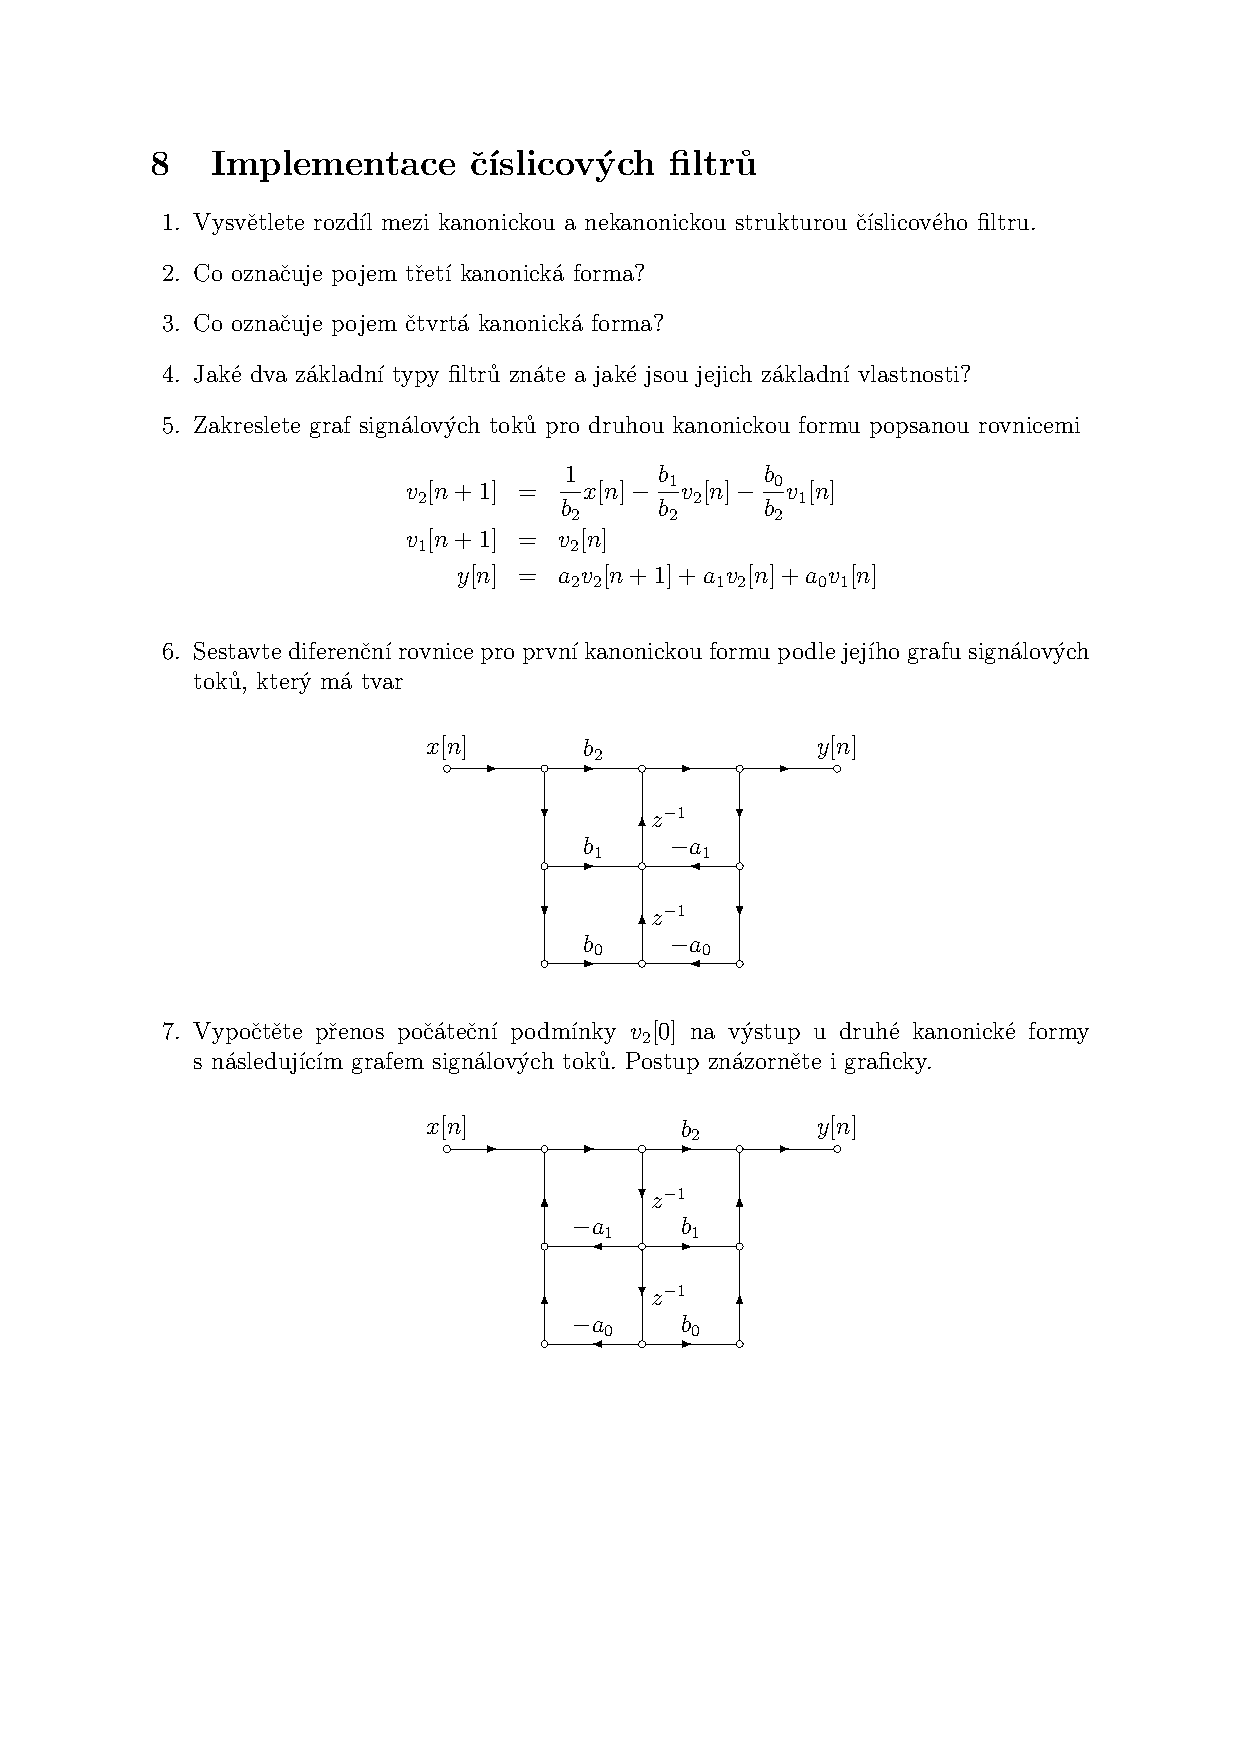
\includepdf[pages =-]{mspr-q07.pdf}
\section{Vliv kvantování na implementaci číslicových filtrů}

\includepdf[pages =-]{mspr-kvantovani.pdf}
\section{Vliv kvantování na implementaci číslicových filtrů-otázky}
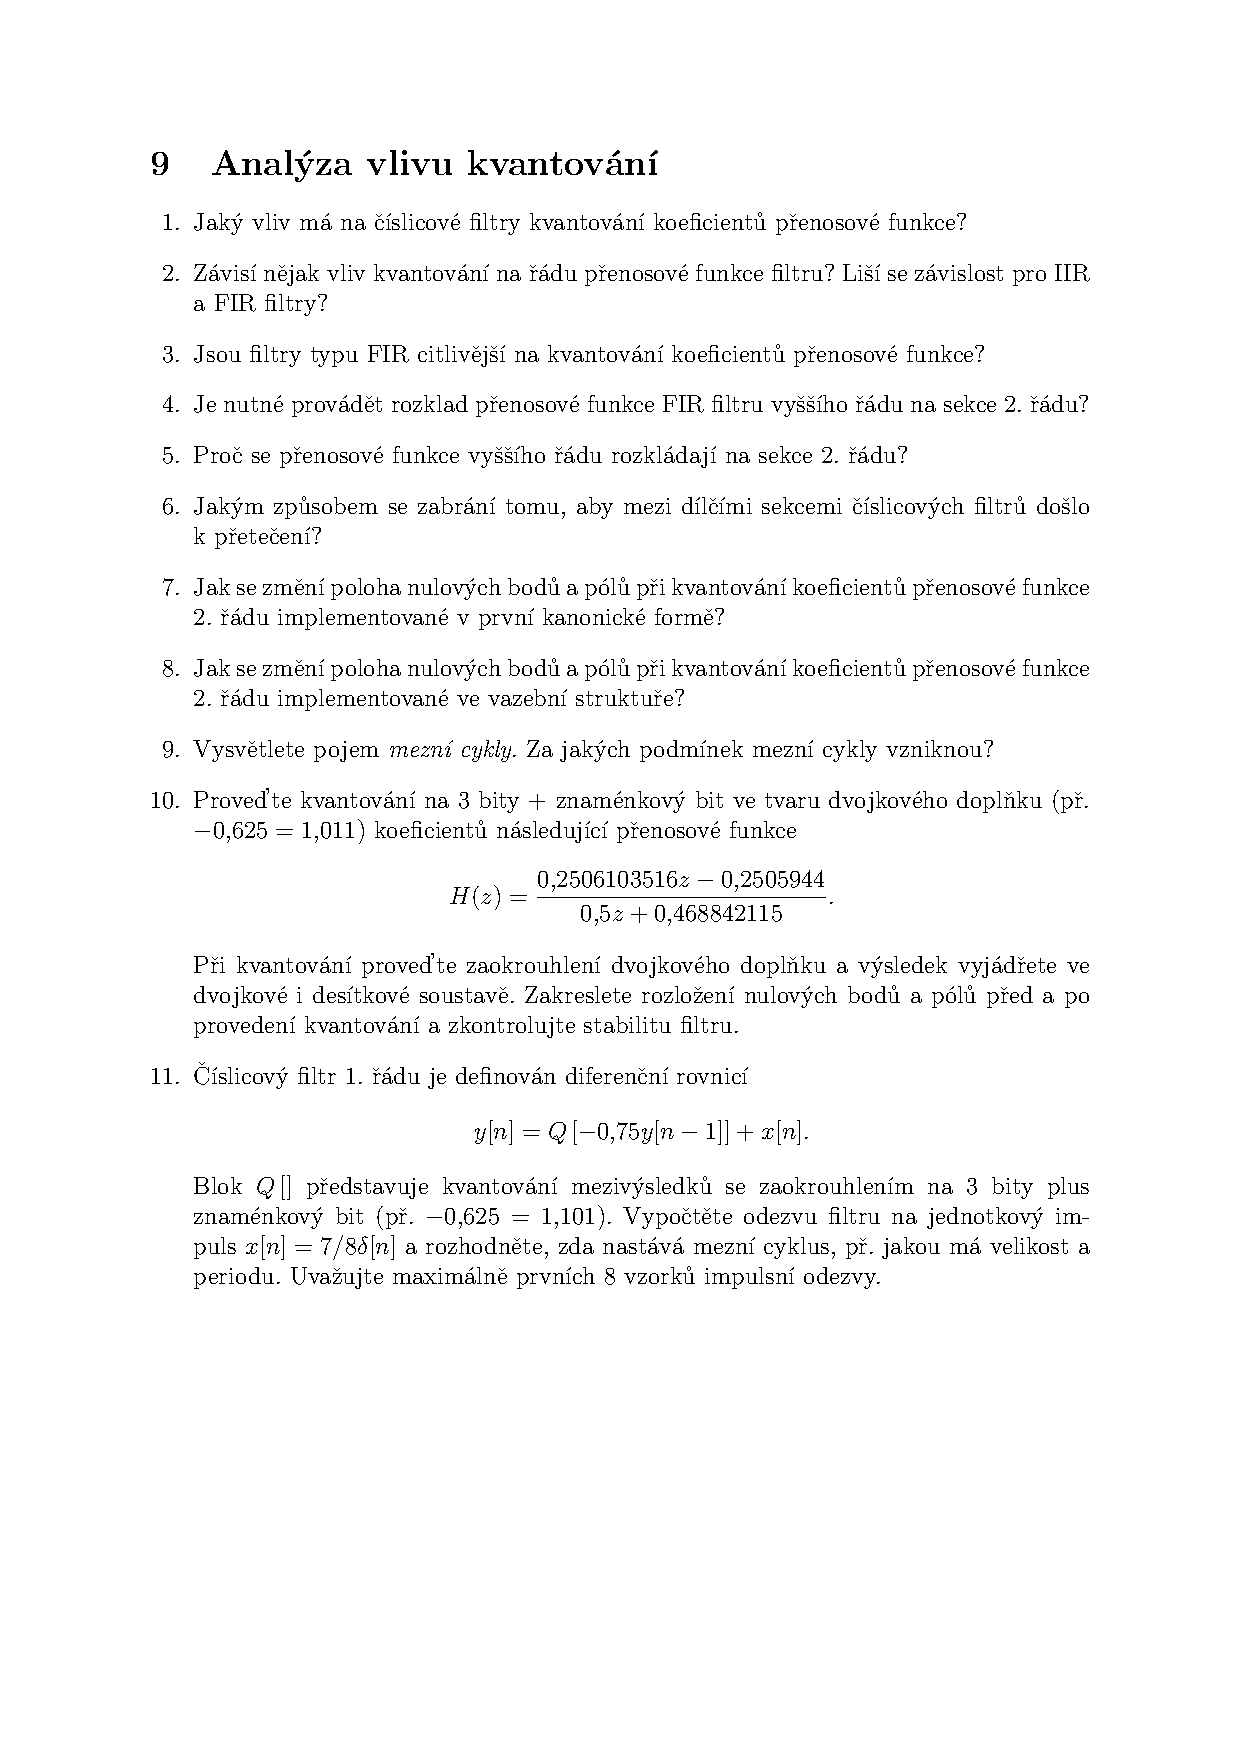
\includepdf[pages =-]{mspr-q08.pdf}
\section{Generace a detekce harmonického signálu}

\includepdf[pages =-]{fft.pdf}
\section{Generace a detekce harmonického signálu-otázky}
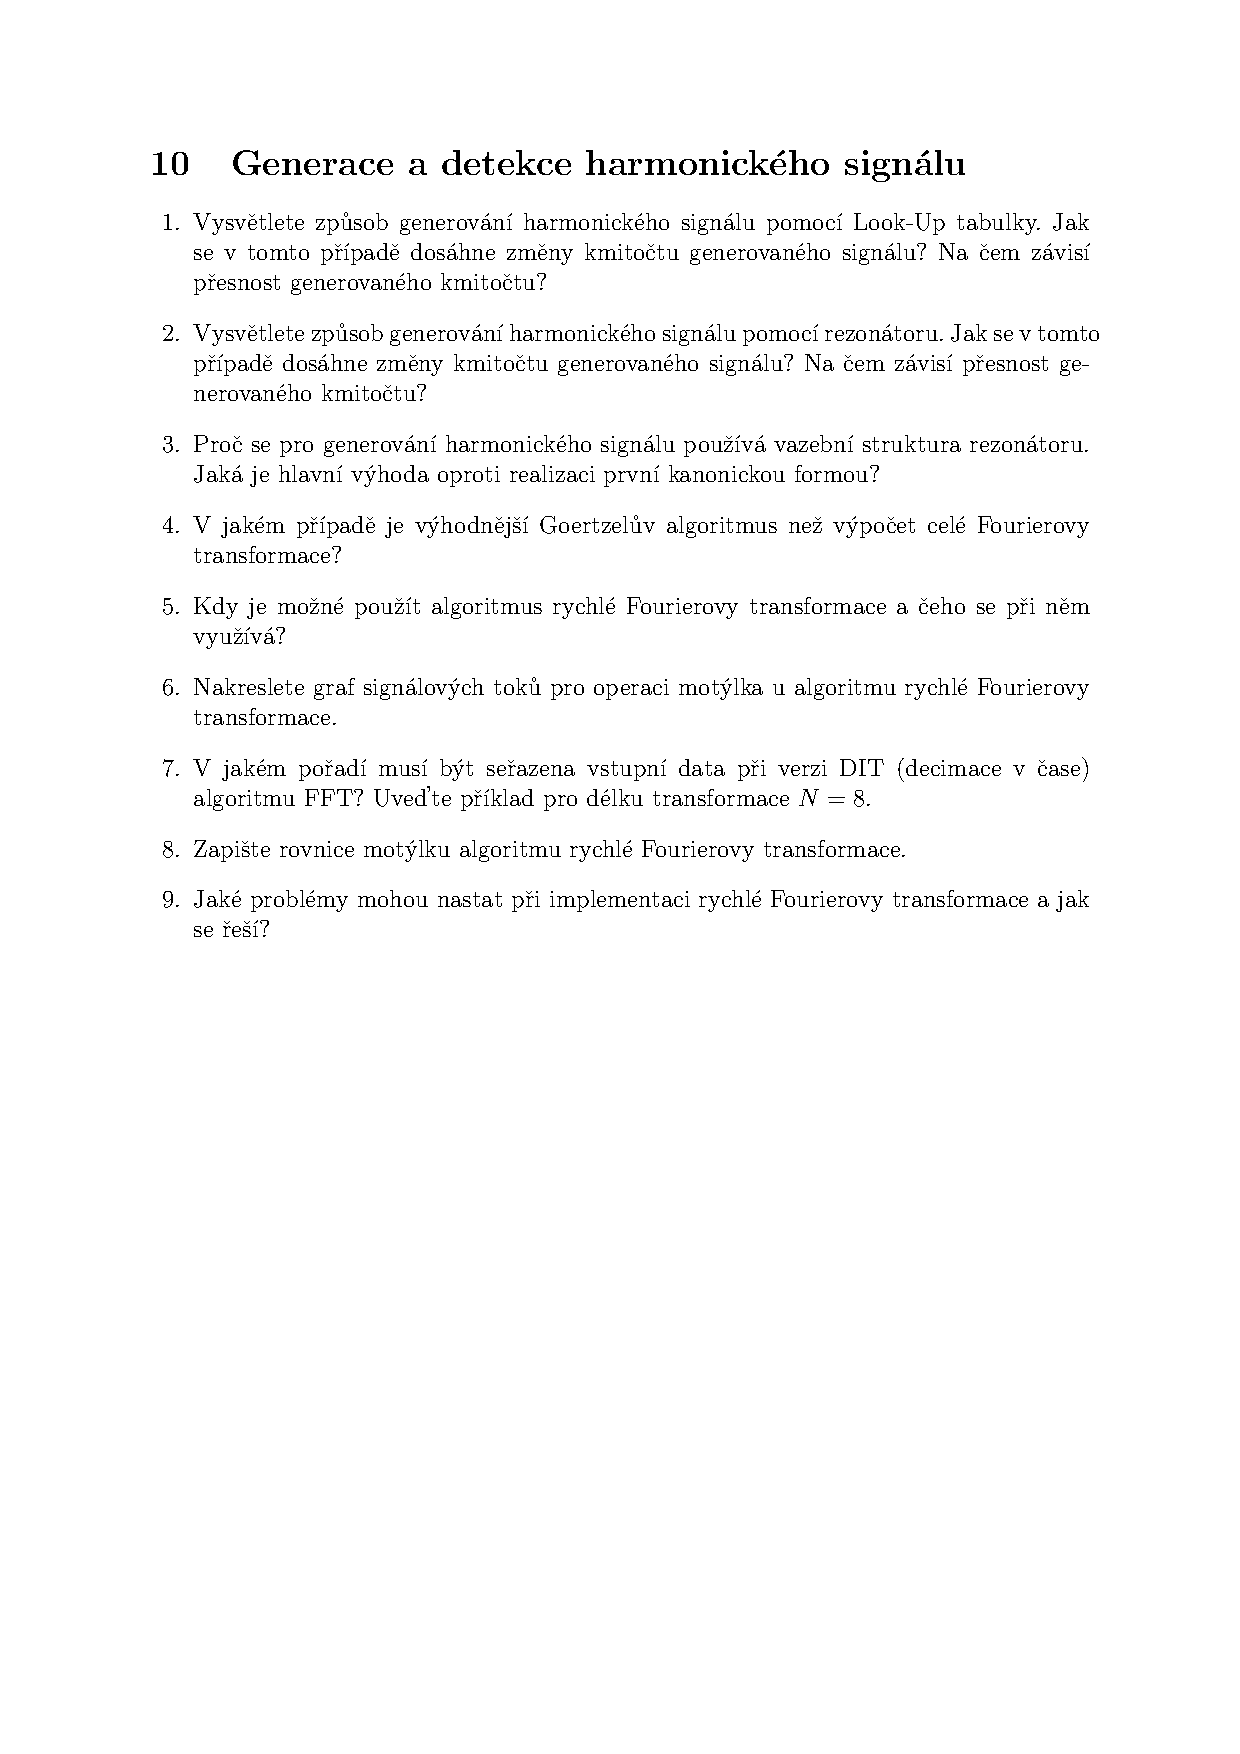
\includepdf[pages =-]{msprq10.pdf}
\section{Řadič programu}

\includepdf[pages =-]{pipelining.pdf}
\section{Řadič programu - otázky}

\includepdf[pages =-]{msprq12.pdf}
\section{Architektury signálových procesorů}

\includepdf[pages =-]{mspr-architektury.pdf}
\section{Vzorkování signálu}
\includepdf[pages =-]{mspr-vzorkovani.pdf}
\section{Vzorkování signálu-otázky}
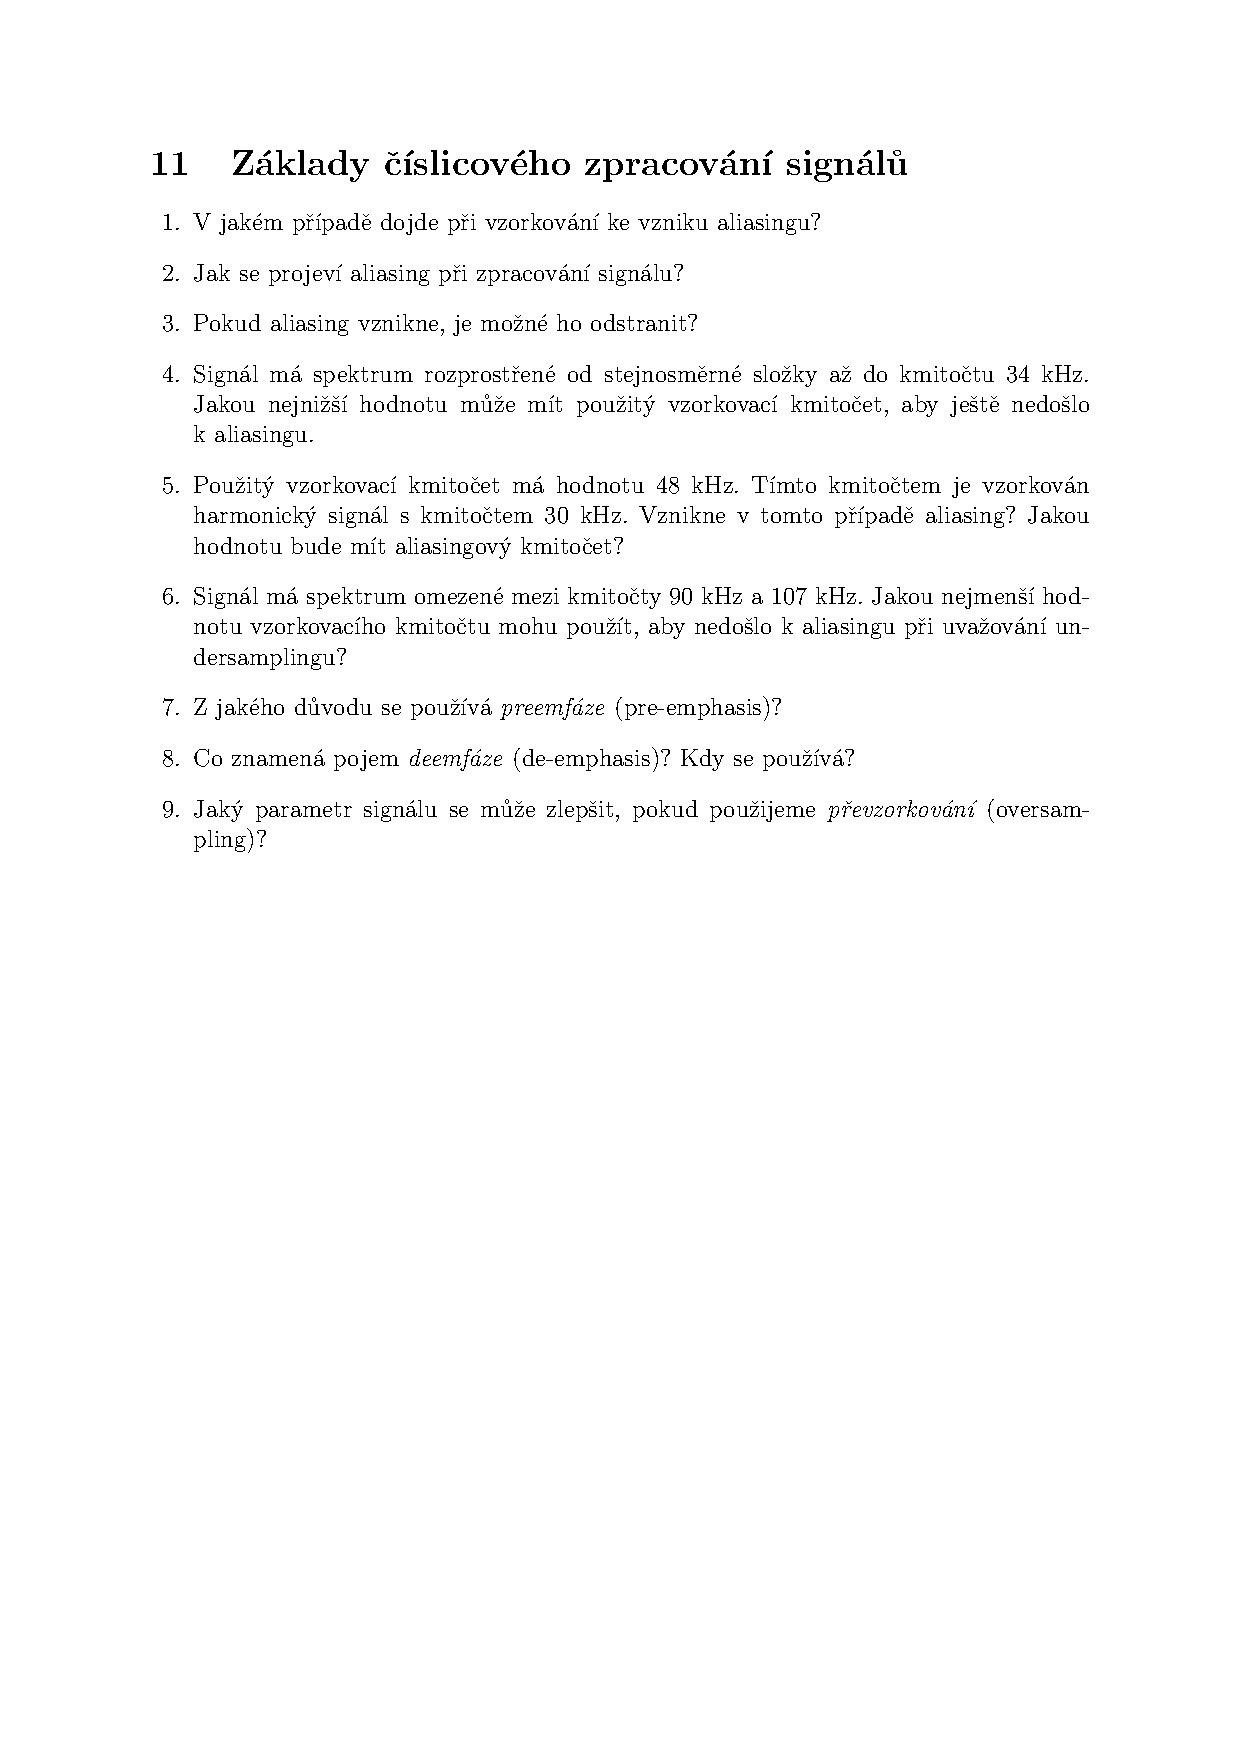
\includepdf[pages =-]{msprq13.pdf}

\end{document}


